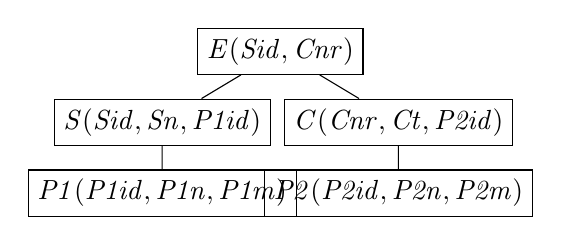
\begin{tikzpicture}[scale=0.6]
    \node	(5)	at	(-2.5,-1)		[align=center,rectangle,draw]	{$\mathit{P1(P1id,P1n,P1m)}$};
	\node	(4)	at	(2.5,-1)		[align=center,rectangle,draw]	{$\mathit{P2(P2id,P2n,P2m)}$};
	\node	(3)	at	(2.5,.5)		[align=center,rectangle,draw]	{$\mathit{C(Cnr,Ct,P2id)}$}
		edge(4);
	\node	(2)	at	(-2.5,.5)	[align=center,rectangle,draw]	{$\mathit{S(Sid,Sn,P1id)}$}
	    edge(5);
	\node	(1)	at	(0,2)		[align=center,rectangle,draw]	{$\mathit{E(Sid, Cnr)}$}
		edge(2)
		edge(3);
\end{tikzpicture}